

\title{Computer Vision Summary}
\author{
        Manuel Galliker  14-921-969 \\
                manuelga@student.ethz.ch
}
\date{\today}

\documentclass[12pt]{article}
\usepackage{graphicx}
\begin{document}
\maketitle


\section{Lectures}
\subsection{Intro and Pinhole Model}
There are many application where computer vision is very usefull. It can be used to relief humans of repetitive tasks, to enhance human abillities, give perception to robots or to organize visual content just to name a few.
\newline
\section{Direct Linear Transform}
As described in the exercise, the DLT Algorithm is used to calibrate the camera. In the beginning, all points are normalized to compute matrix $A$, which is calculated with the respective 2D and 3D points. The results of the different points are then appended underneath the existing matrix. This results in a Matrix $A$ which yields zero is multiplied with the projection matrix.
 $AP=0$
 Therefore, P is the null-vector of A, which can be found using the Singular Value Decomposition. In the end, $P$ gets denormalized to continue with the QR-Decomposition.
\newline
 $ P = \left[ \begin{array}{rrrr}
 77.3584  & -3.3989 & -12.7338 &-570.8504 \\
 25.6914 &  42.2237 &  53.6358 &-743.6380 \\
 0.0251  &  0.0401 &  -0.0170  & -0.6581 \\
 \end{array}\right] $
\vspace{5mm}
\newline
The QR-Decomposition of $P$ results in the intrinsic Camera matrix $K$, the Rotation Matrix $R$ and the camera center $C$:
\vspace{5mm}
\newline

$ K = \left[ \begin{array}{rrr}
-0.0005 &   0.0002 &   0.0003\\
0  &  0.9101  &  0.1885\\
0     &    0   & 1.0000\\
\end{array}\right] $
\vspace{5mm}
\newline
$ R = \left[ \begin{array}{rrr}
0.9820 &  -0.1780 &  -0.0634\\
-0.1859  & -0.9702 &  -0.1555\\
-0.0338 &   0.1645 &  -0.9858\\
\end{array}\right] $
\vspace{5mm}
\newline
$ t = \left[ \begin{array}{r}
-5.7418\\
12.9930\\
-0.8810\\
\end{array}\right] $
\vspace{5mm}
\newline
$Error =    2.3907$

\begin{figure}[ht]
	\centering
  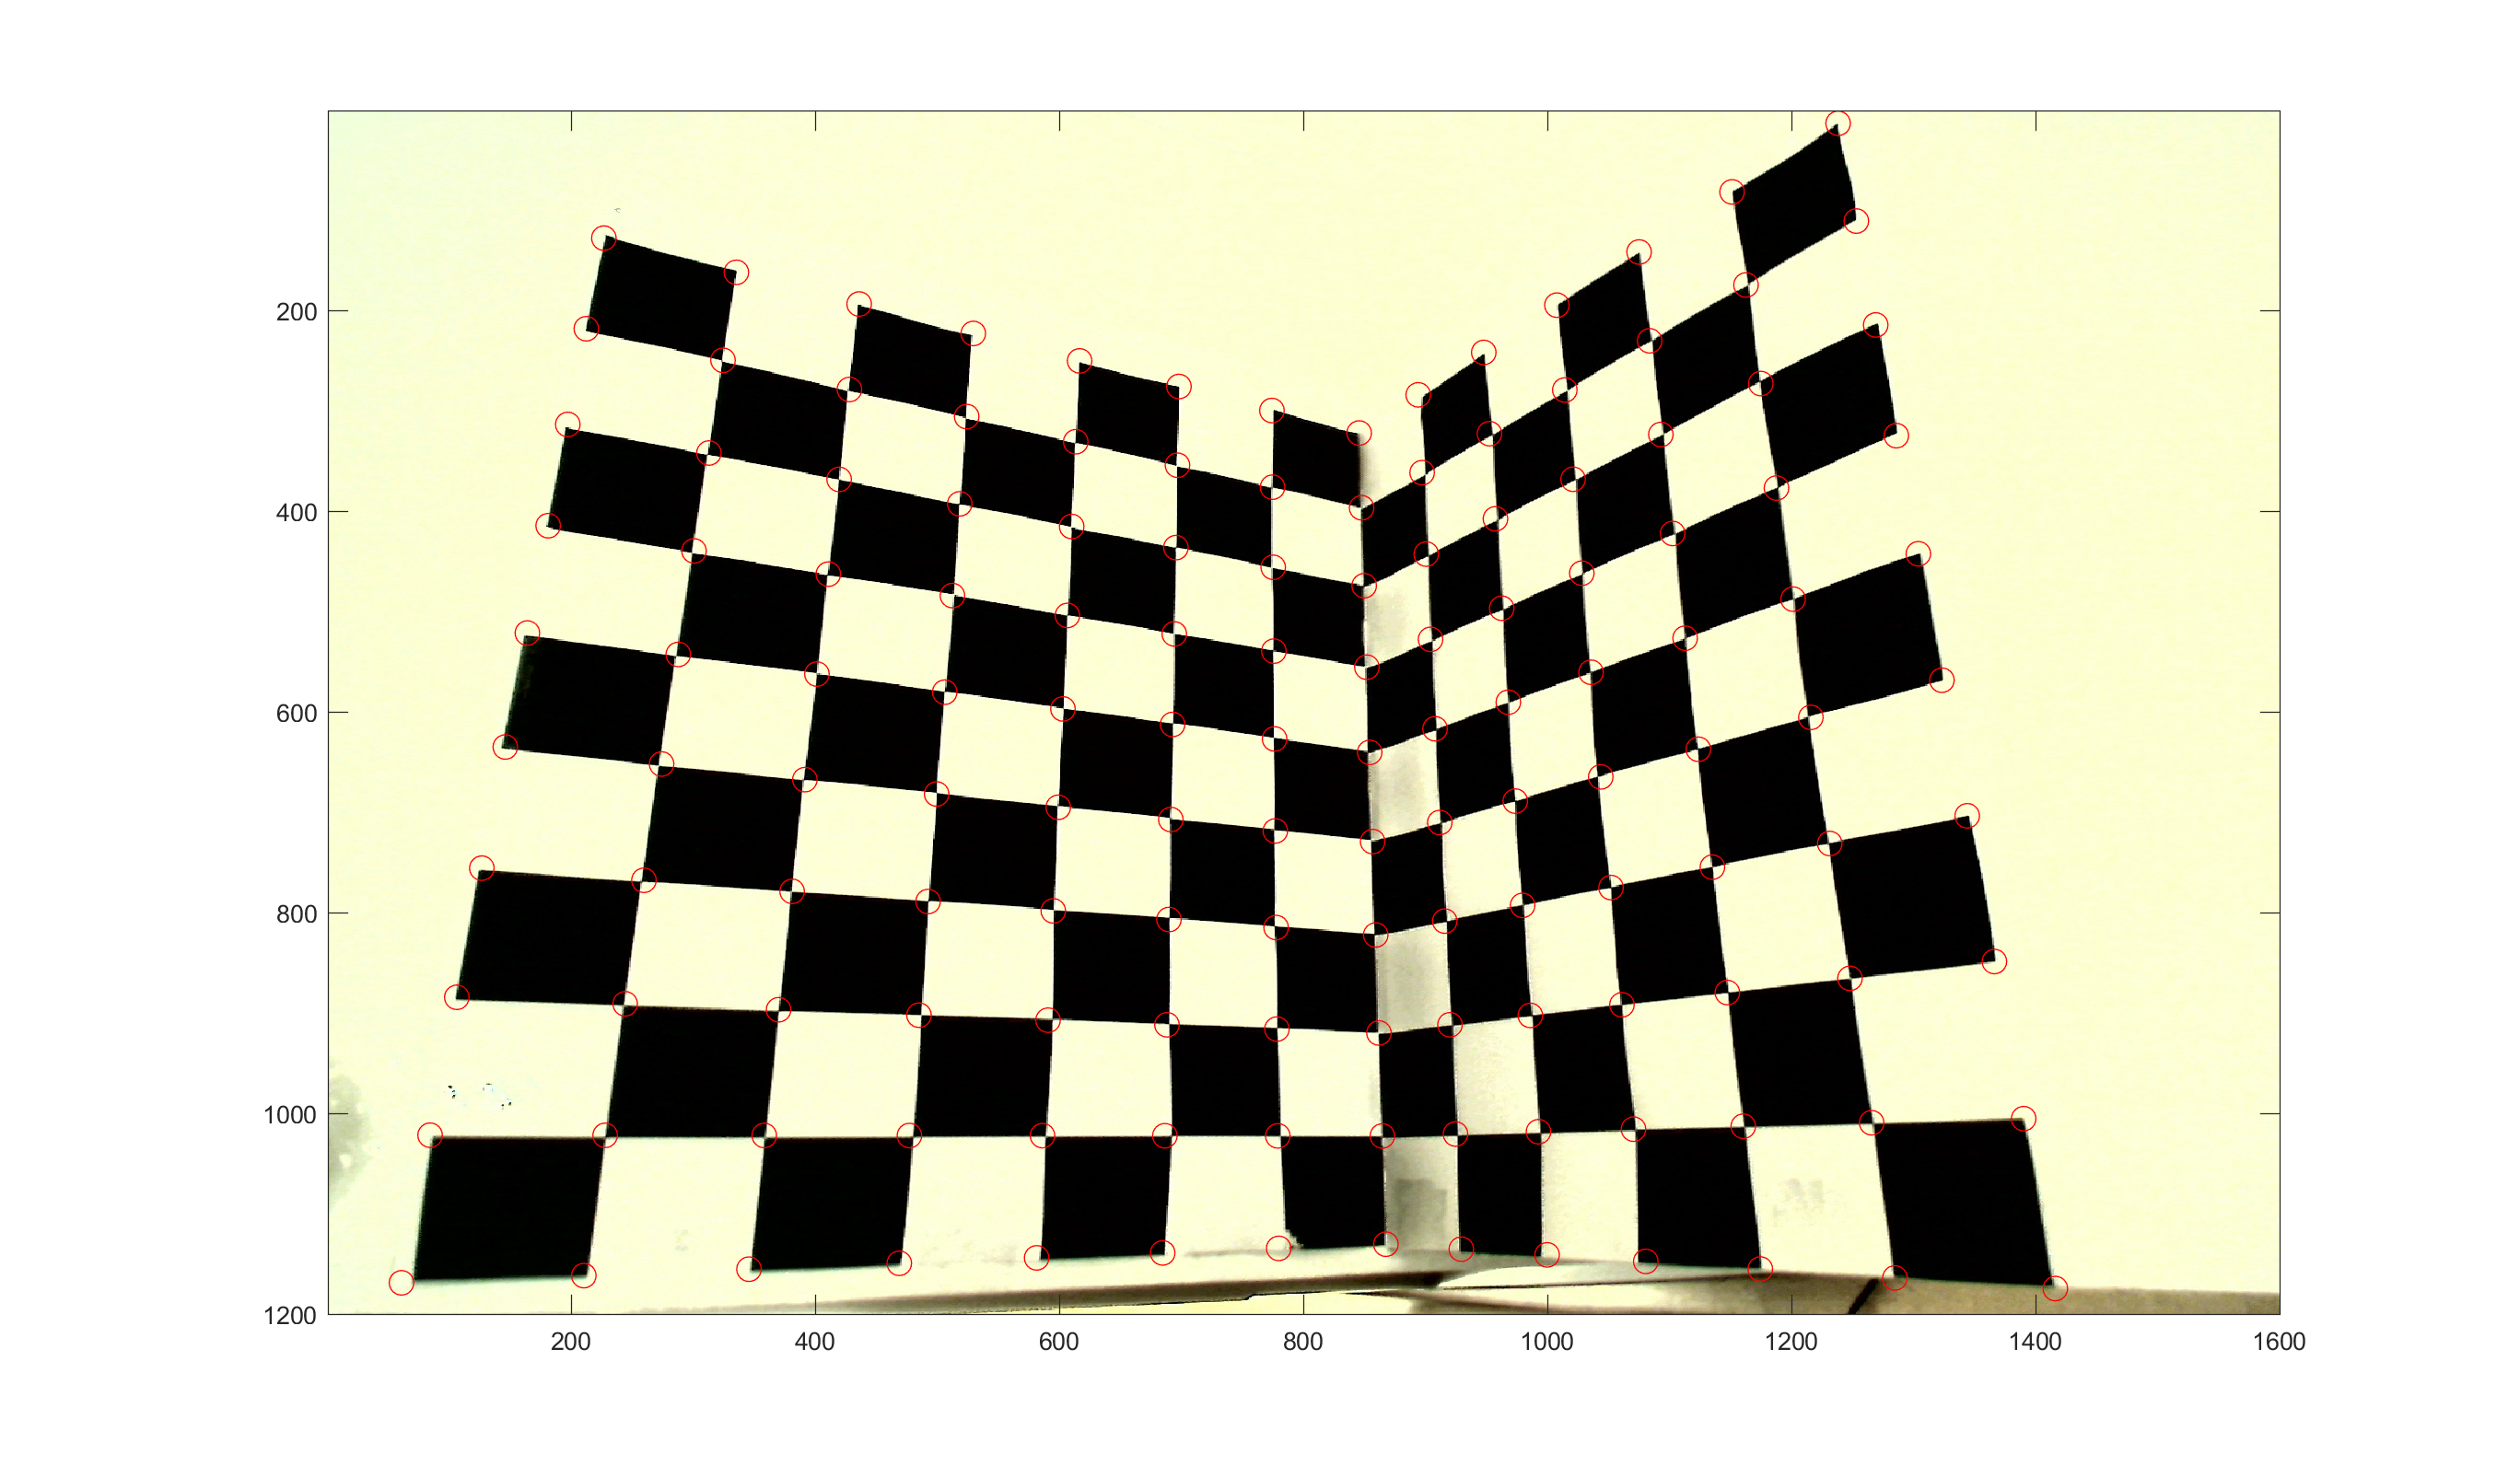
\includegraphics[width=0.9\textwidth]{dlt_reprojected_points1.png}
	\caption{DLT: Reprojected Chess Board Corners}
	\label{fig1}
\end{figure}

\begin{figure}[ht]
	\centering
  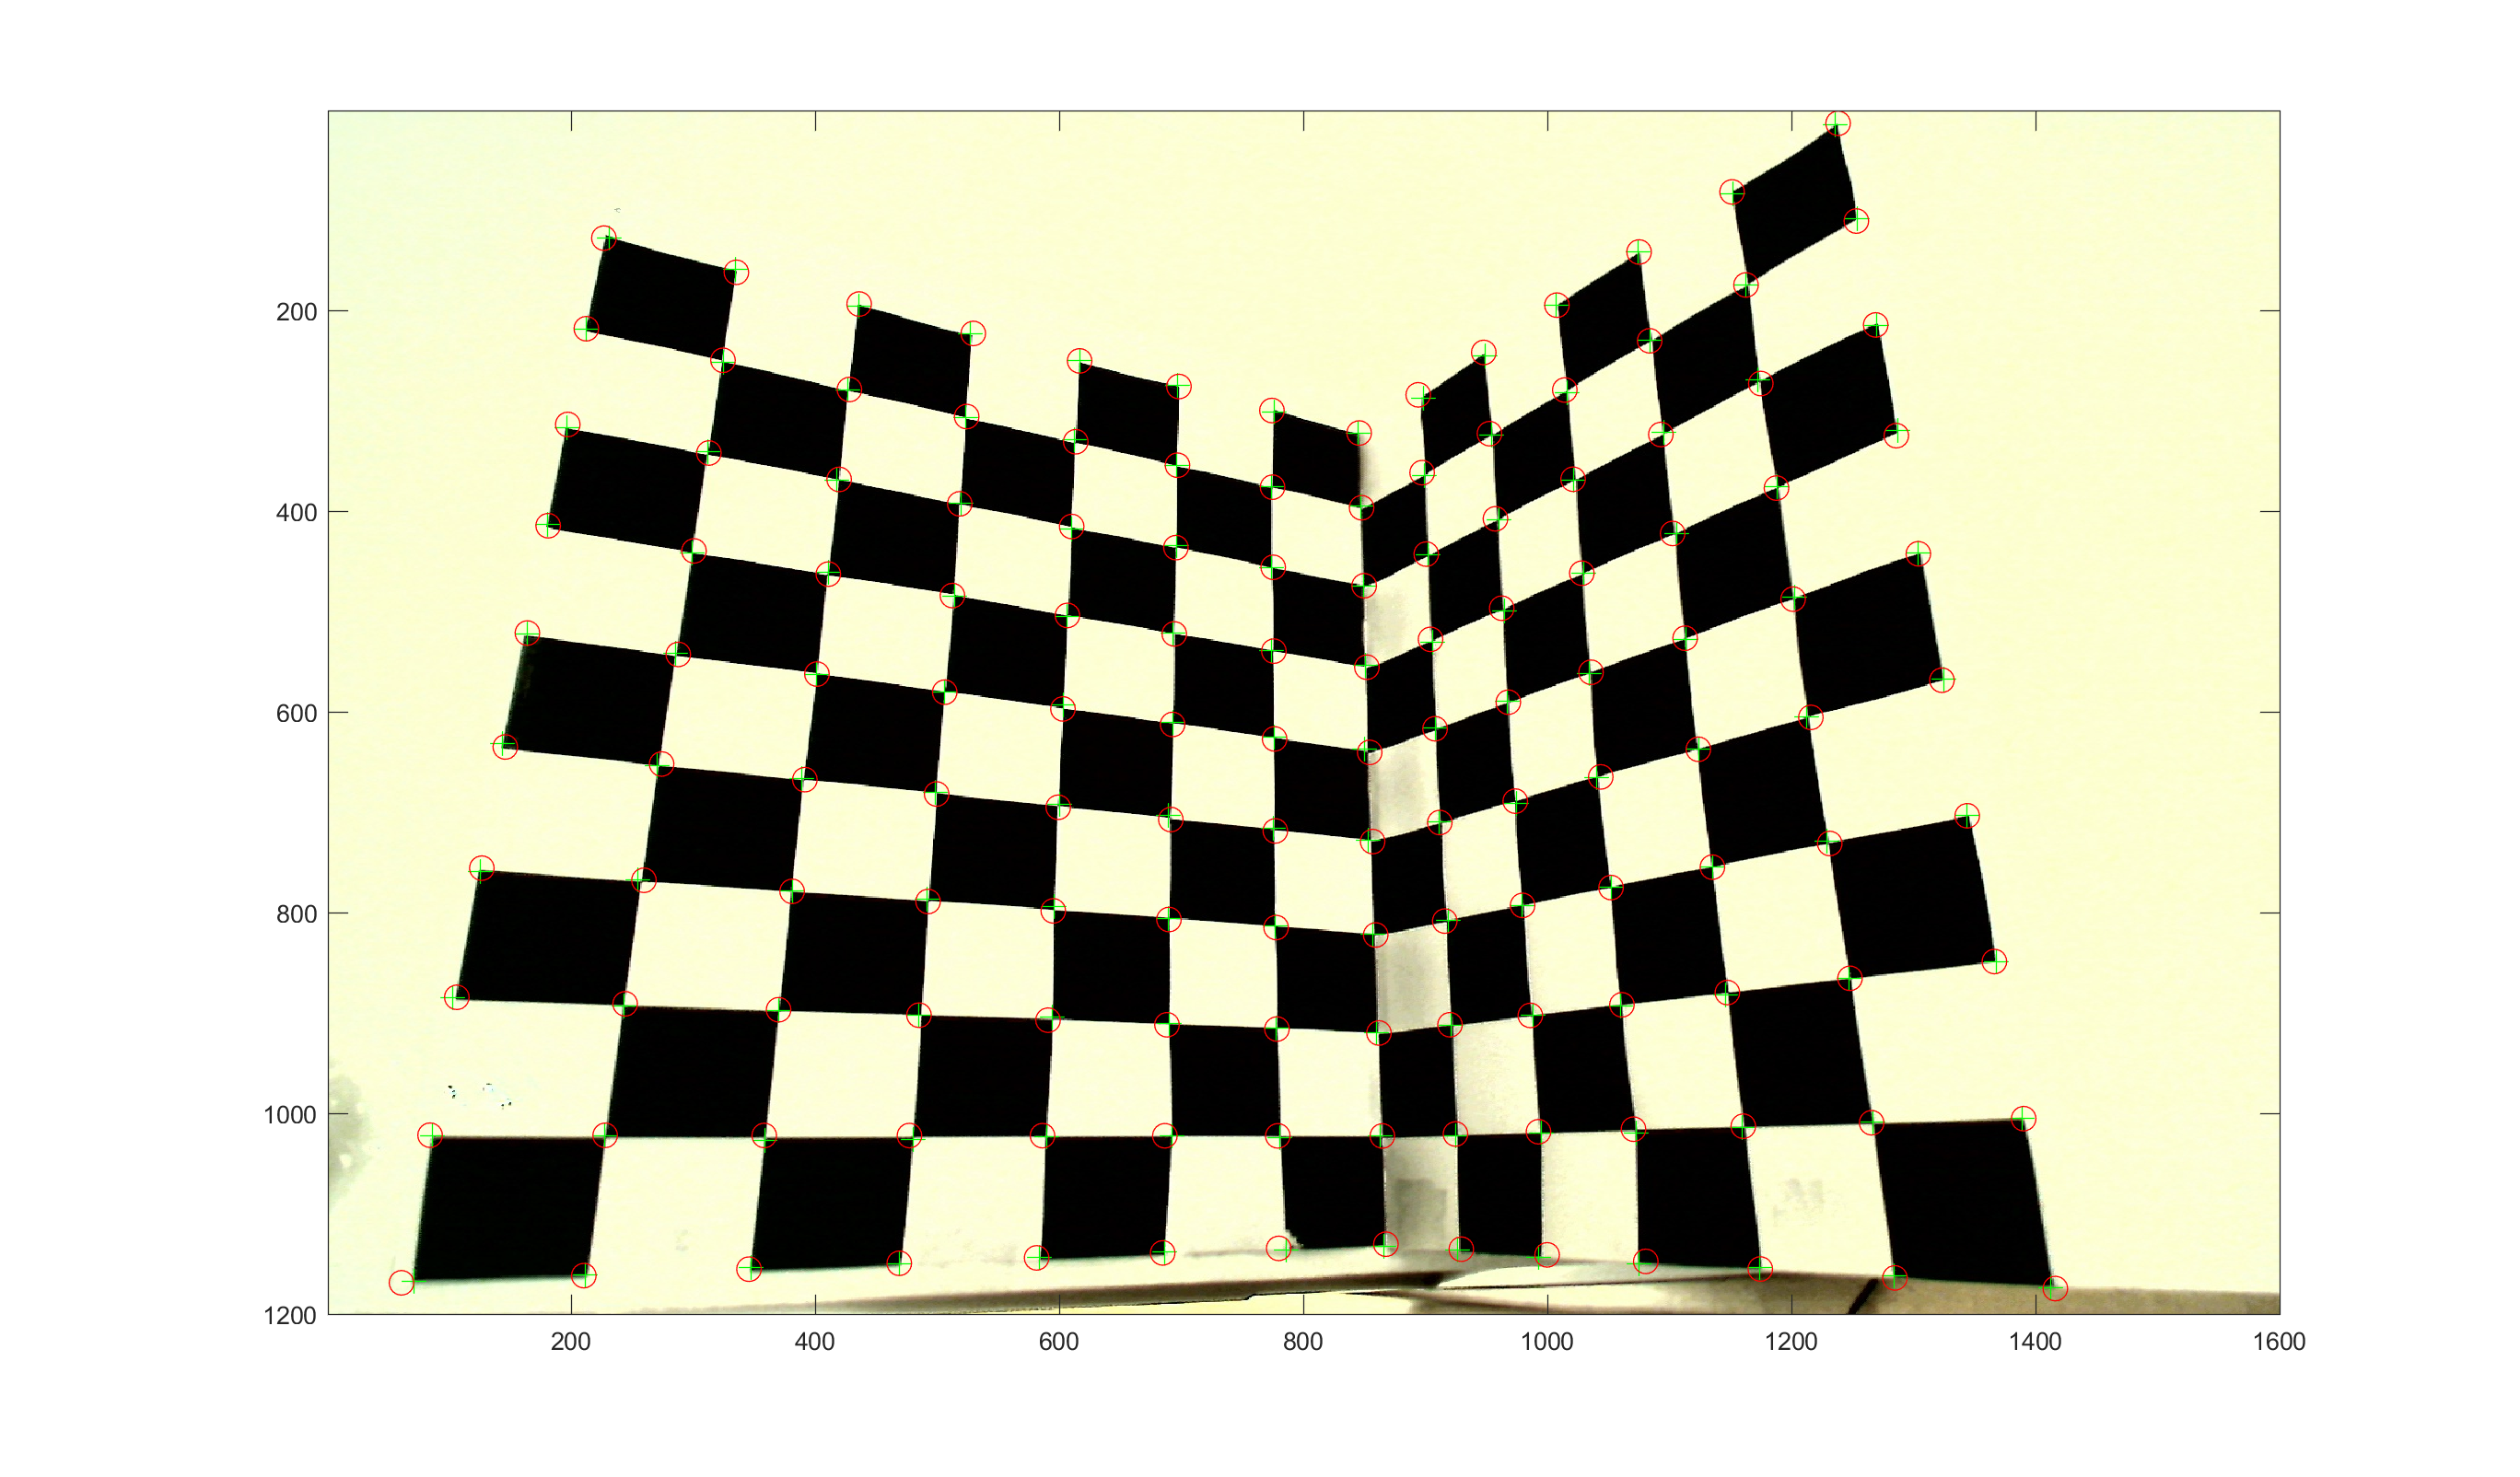
\includegraphics[width=0.9\textwidth]{dlt_all_points1.png}
	\caption{DLT: Original and Reprojected Chess Board Corners}
	\label{fig1}
\end{figure}

If xy and XYZ are not normalized before applying the Direct Linear Transform the error is slightly smaller:
\vspace{5mm}
\newline
$Error =    2.3880$
\vspace{5mm}
\newline
This means that with the used dataset all calculations have to be far away from any singularities. It seems that for this specific dataset a normalization would not have been needed. Nevertheless, one datapoint is far not enough for a generalized conclusion. 

\section{Gold Standard Algorithm}
The Golden Standard uses the DLT Algorithm as an basis to improve opon. $P_normalized$ is iteratively improved with the optimization algorithm fminsearch to reduce the reprojection error. Same as in DLT, points are normalized and denormalized before and after the calculation. 
\vspace{5mm}
\newline
$ P = \left[ \begin{array}{rrrr}
77.2903  & -3.5770 & -12.6734 & -570.6325 \\
25.6226  & 42.1398 &  53.6676 & -743.5304 \\
0.0250   & 0.0400  & -0.0169  & -0.6580 \\
\end{array}\right] $
\vspace{5mm}
\newline
$ K = \left[ \begin{array}{rrr}
-0.0005 &   0.0002  &  0.0003 \\
0  &  0.9106  &  0.1870 \\
0   &      0  &  1.0000 \\
\end{array}\right] $
\vspace{5mm}
\newline
$ R = \left[ \begin{array}{rrr}
0.1420  & -0.9880 &  -0.0611 \\
-0.9790  & -0.1310  & -0.1564 \\
0.1466   & 0.0820 &  -0.9858 \\
\end{array}\right] $
\vspace{5mm}
\newline
$ t = \left[ \begin{array}{r}
10.5131 \\
9.5474 \\
-1.3733 \\
\end{array}\right] $
\vspace{5mm}
\newline
$Error = 2.3681$
\vspace{5mm}
\newline
As can be seen the error is smaller than with normalized and unnormalized LTR. 

\begin{figure}[ht]
	\centering
	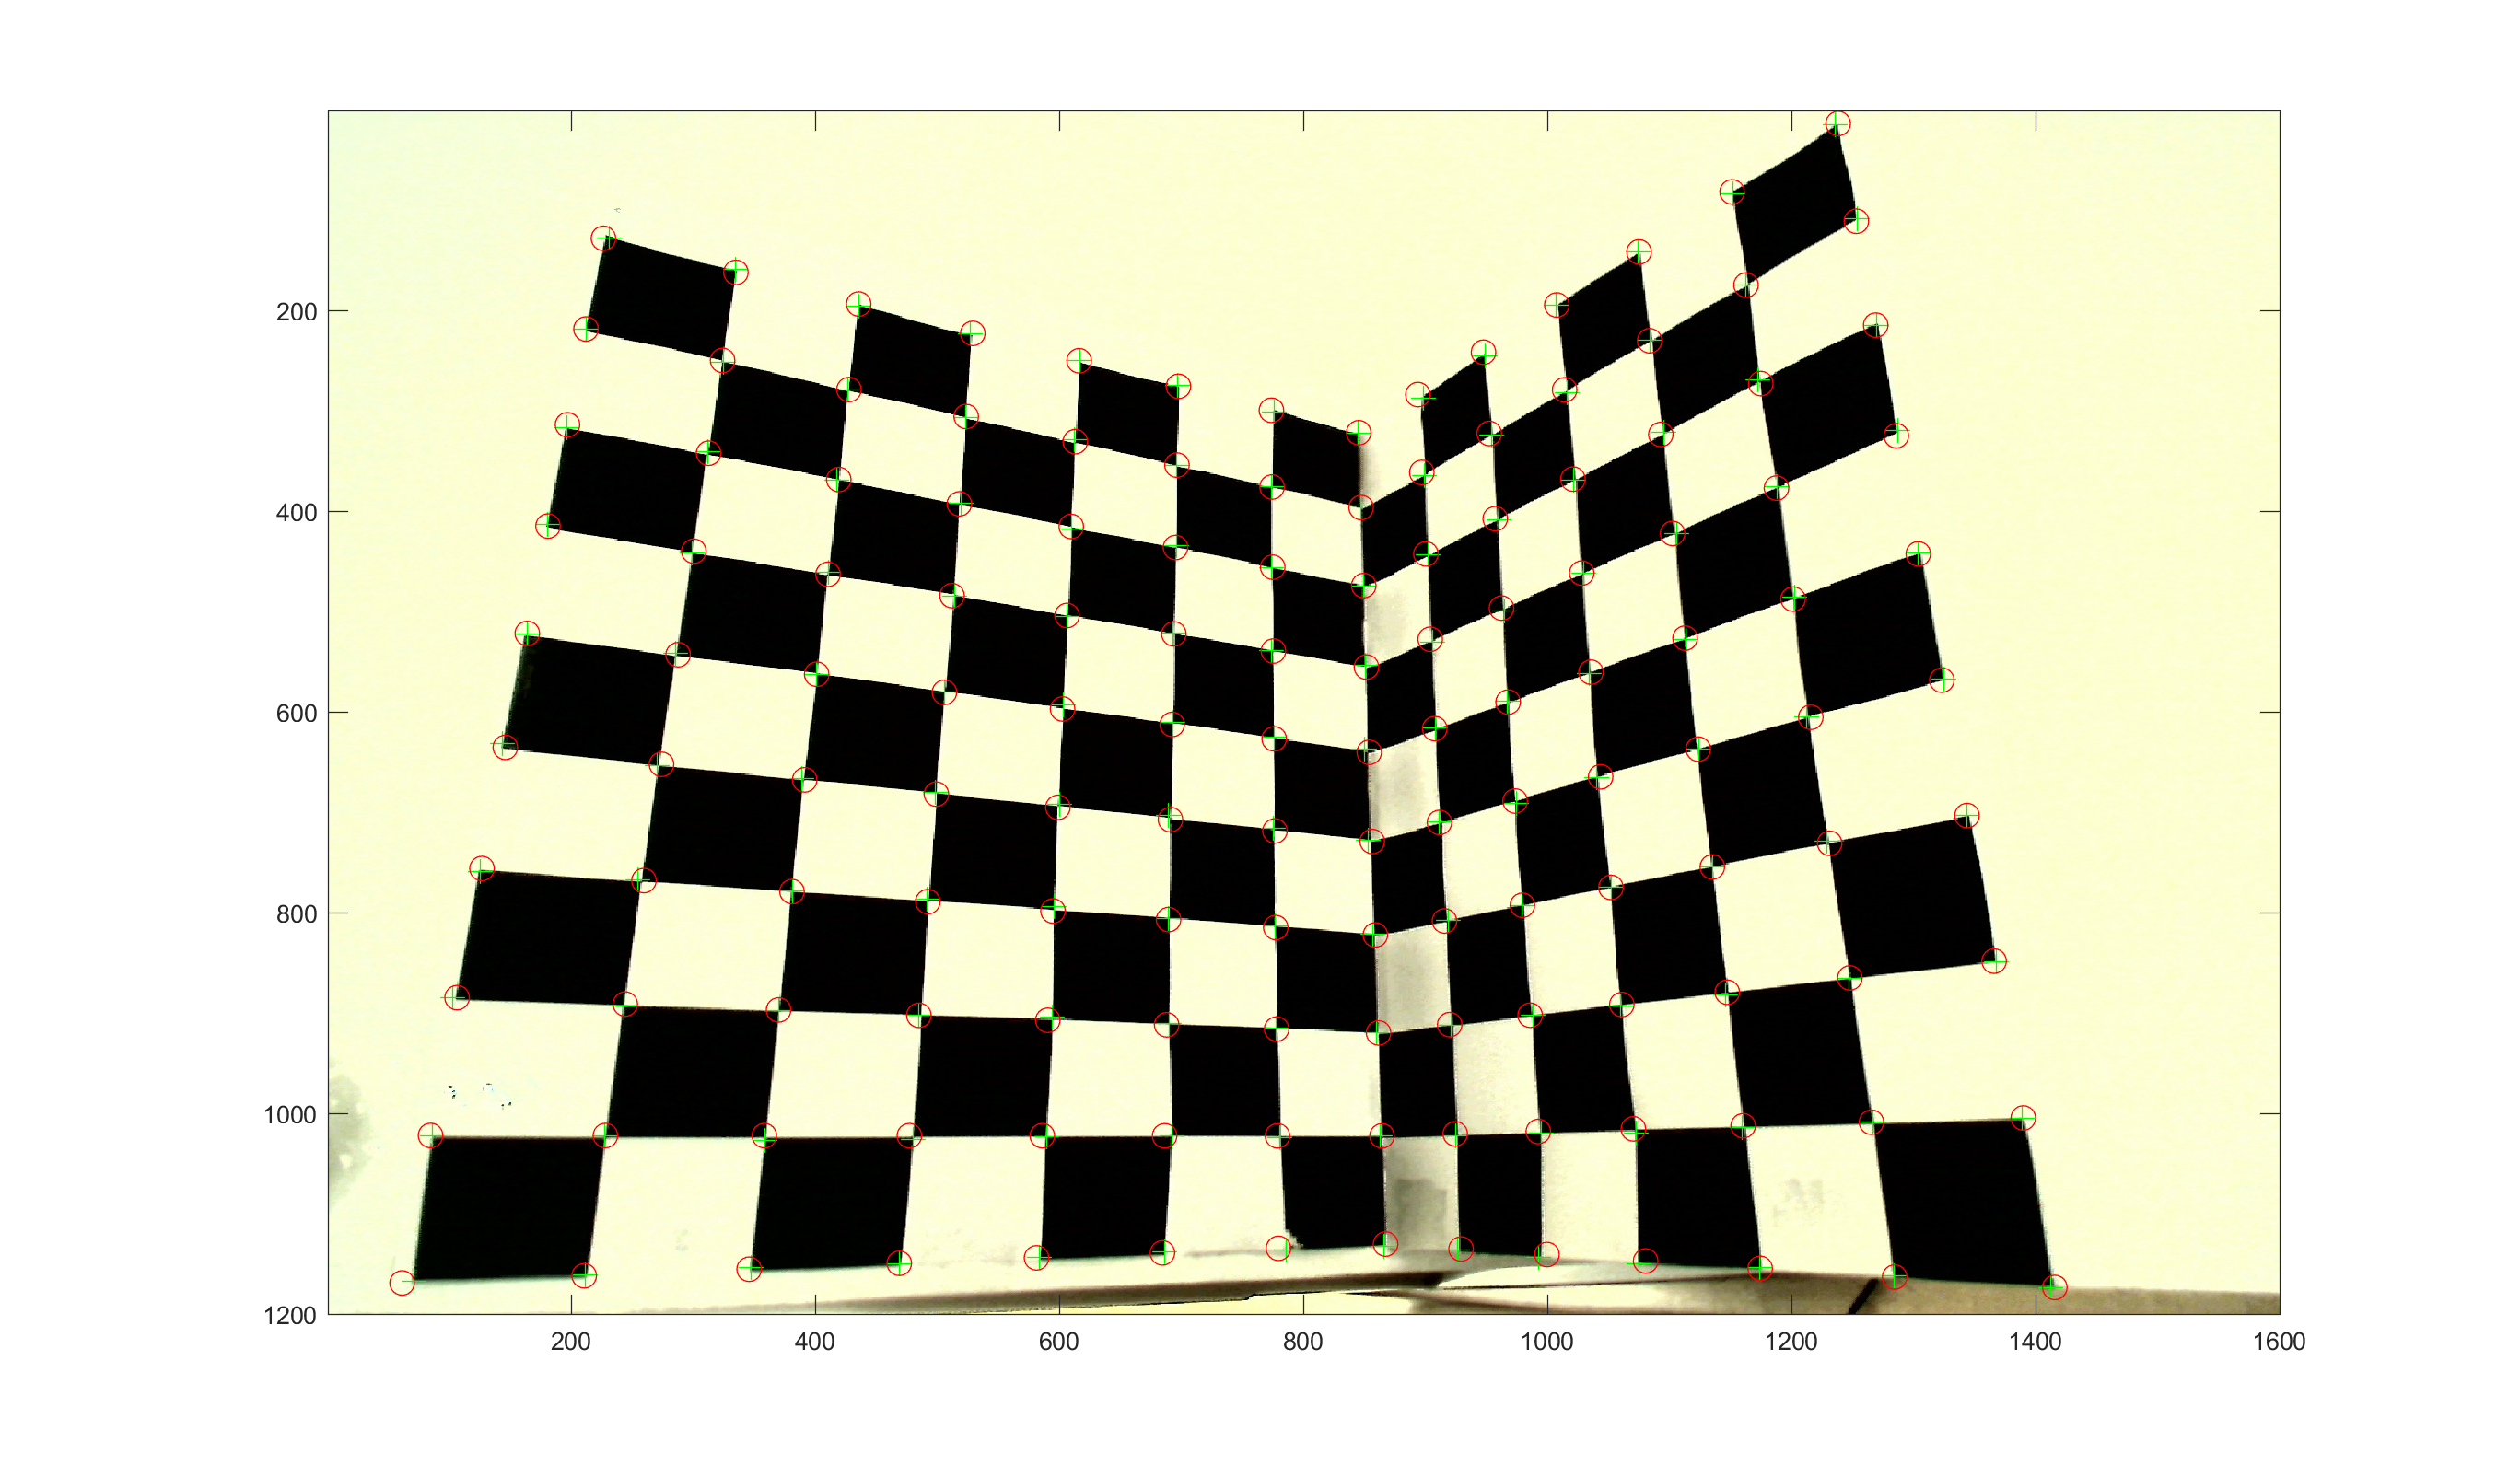
\includegraphics[width=0.9\textwidth]{gold.png}
	\caption{GSA: Original and Reprojected Chess Board Corners}
	\label{fig1}
\end{figure}

\section{Discussion}
As could be seen the LTR method gives already very accurate reprojections of points. This results can be further improved with the Golden Standart optimization algorithm. 
\vspace{5mm}
\newline
Unexpectatly the not normalized LTR yielded slightly better results than the normalized LTR algorithm. As has been observed the normalization algorithm doesn't yield perfect results due to numerical rounding. It was observed, that for example the mean offset after normalization could still be in the order of magnitude of $10^-14$. This might be a possible explanation for the slightly better performance of the non normalized LTR in this case.

\end{document}